%
% einleitung.tex -- Beispiel-File für die Einleitung
%
% (c) 2020 Prof Dr Andreas Müller, Hochschule Rapperswil
%
% !TEX root = ../../paper.tex
% !TEX encoding = UTF-8
%
\section{Geschichte\label{geostrophisch:section:teil0}}
\kopfrechts{Geschichte}

Lewis Fry Richardson war ein britischer Meteorologe und Friedensforscher.
Schon sehr früh in seinem Leben entdeckte er seine Passion für die Mathematik. 
In den 1910er Jahren entwickelte er eine aussergewöhnliche Methode, um analytisch nicht lösbare Partielle Differentialgleichungen zu lösen.
Anschliessend veröffentlichte er einen Artikel, in welchem er diese Methode erklärte.
Nach dieser Veröffentlichung studierte er über die Anwendung der Methode auf das Problem der Wettervorhersage. 

Die Anfänge der numerischen Wettervorhersage gehen auf den britischen Mathematiker und Physiker \textbf{Lewis Fry Richardson} (1881–1953) zurück.  
In seinem Werk \textit{Weather Prediction by Numerical Process} (1922) formulierte Richardson als Erster die Idee, eine numerische Wettervorhersage durch das explizite Lösen eines physikalisch fundierten Gleichungssystems zu bestimmen.  
Damit legte er den theoretischen Grundstein für die moderne Wettermodellierung.

\begin{figure}[h]
	\centering
	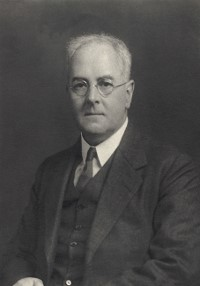
\includegraphics{Portrait_Richardson.jpg}
	\caption{text}
	\label{bild:portraitRichi}
\end{figure}

Siehe ~\ref{bild:portraitRichi} das ist ein Portrait Foto von Richardson.

\begin{itemize}
	\item \textbf{Bewegungsgleichungen:} Horizontale und vertikale Impulsbilanz
	\item \textbf{Kontinuitätsgleichung:} Erhaltung der Masse
	\item \textbf{Energiegleichung:} Thermodynamische Prozesse
	\item \textbf{Zustandsgleichung:} Zusammenhang zwischen Druck, Temperatur und Dichte
\end{itemize}






